To address the research questions posed in~\autoref{sec:research-questions}, it is imperative to first comprehend the subjects and their fundamentals. 

We start by defining  and giving an overview of the topic areas touched upon by this thesis~(\autoref{sec:defs}) and their theory,  and then explain the technologies used within the tool ExpoSE ~(\autoref{sec:defs}).

\section{Terminology and Theory}
\label{sec:defs}
To provide an overview of all the topics that will be addressed, we will begin by defining the key components of this thesis and explaining the basics to build upon in the later chapters. 

\subsection{Web Applications}
\label{sec:webapp}
A \textit{web application} has been defined as “a software application, executed by a web server, which responds to dynamic web page requests over HTTP” by the Web Application Security Consortium (WASC) ~\cite{noauthor_web_2012}. 
In simpler terms, a web application is software that runs on a server and users access it through a web browser (like Chrome or Firefox) over the internet.

Typically, the resources and scripts of web applications — such as images, text, or functionalities — are requested by the client, which is the user's computer or device, using a web browser or similar tools. This interaction follows a set of rules known as the \gls{api}, which specifies what requests can be made and how the server should respond.
The~\autoref{fig:simplified-web-app} illustrates the basic communication process between the client (the user's device), the server (where the application runs), and external services (such as another server).

Most web applications also use a database, which is a structured way of storing data, to keep information consistently available and reliable. For the purposes of this thesis, we assume that the web application has a monolithic architecture. This means that it operates as a single cohesive program on a physical computer, rather than being divided into separate parts that run on different cloud services (like AWS, or Amazon Web Services, which offers online computing power without needing dedicated hardware\footnote{https://aws.amazon.com/})
Additionally, we assume the server follows REST (Representational State Transfer) principles, which are guidelines for how web services should operate to enable smooth communication as described by \citet{roy_t_fielding_rest_2008}. 
The web server processes requests that adhere to the HTTP (Hypertext Transfer Protocol) standard, which is the foundational protocol used for transmitting data on the web (ref. ~\autoref{tab:rest_http_methods}). It can be used  with the database operations, commonly known as CRUD (Create, Read, Update, Delete) operations, as established by \citet{martin_managing_1983}, when a web application utilizes a persistent database.
This adherence ensures that the server and client can operate independently, meaning they can be developed and updated separately without affecting each other\cite{fielding_http_2022}.


\begin{figure}[ht]
    \centering
    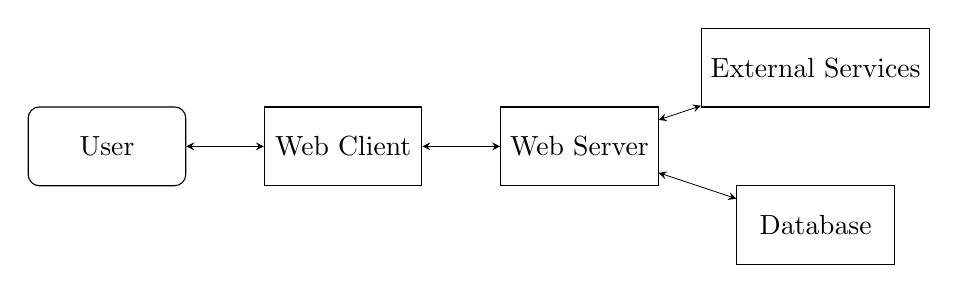
\begin{tikzpicture}[node distance=3cm]
    % Define styles for nodes and arrows
    \tikzstyle{user} = [rectangle, rounded corners, minimum width=2cm, minimum height=1cm, text centered, draw=black]
    \tikzstyle{browser} = [rectangle, minimum width=2cm, minimum height=1cm, text centered, draw=black]
    \tikzstyle{server} = [rectangle, minimum width=2cm, minimum height=1cm, text centered, draw=black]
    \tikzstyle{database} = [rectangle, minimum width=2cm, minimum height=1cm, text centered, draw=black]
    \tikzstyle{external} = [rectangle, minimum width=2cm, minimum height=1cm, text centered, draw=black]
    % Use arrows with both directions
    \tikzstyle{arrow} = [thick, <->, >=stealth]
% Arrow style for double lines

    \tikzset{doubleArrow/.style={thick, <->, >=stealth,
        line width=0.1mm, line cap=round, draw=black
    }}
    % Nodes
    \node (user) [user] {User};
    \node (browser) [browser, right of=user] {Web Client};
    \node (server) [server, right of=browser] {Web Server};
    \node (database) [database, right of=server, yshift=-1cm] {Database};
    \node (external) [external, right of=server, yshift=1cm] {External Services};
    % Arrows (connections)
    \draw  [doubleArrow](user) -- (browser);
    \draw  [doubleArrow](browser) -- (server);
    \draw  [doubleArrow](server) -- (database);
    \draw [doubleArrow] (server) -- (external);
    \end{tikzpicture}
    \caption{Structure of a simplified Web Application}
    \label{fig:simplified-web-app}

\end{figure}

\begin{table}[htb]
    \centering
    \begin{tabular}{@{}lll@{}}
        \toprule
        \textbf{HTTP Method} & \textbf{Purpose}                         & \textbf{Idempotent} \\ \midrule
        GET                   & Retrieve a resource                     & Yes                 \\
        POST                  & Create a new resource                   & No                  \\
        PUT                   & Update or create a resource             & Yes                 \\
        PATCH                 & Partially update a resource             & Yes (mostly)        \\
        HEAD                  & Retrieve headers of a resource         & Yes                 \\
        OPTIONS               & Return available HTTP methods           & Yes                 \\
        DELETE                & Remove a resource                       & Yes                 \\ \bottomrule
    \end{tabular}
    \caption{Summary of REST HTTP Methods and their idempotence \cite[chapter 9]{fielding_http_2022}}
    \label{tab:rest_http_methods}
\end{table}
\FloatBarrier
\subsection{Testing}
\label{sec:testing}

The next aspect we would like to concentrate on is the testing of a web application. First we define what "testing" means, then look into the methodology of "fuzzing" as a technique used to test. We limit this to the following two testing paradigms:
Black Box Fuzzing (\autoref{sec:black-box})and White Box Fuzzing (\autoref{sec:white-box}) .

\subsubsection{Testing}
At its essence, \textit{Testing} constitutes the systematic process of validating and verifying the functionality of a program. A sensible analogy for the concepts of validation and verification was articulated by \citet{b_w_boehm_verifying_1984}:

\begin{itemize}[label={}]
    \item \textit{Verification}: “Am I building the product right?” 
    \item \textit{Validation}: “Am I building the right product?”
\end{itemize}
Depending on the nature of the testing methodology employed, different levels of  assessment can be achieved. A unit test, which is designed to evaluate a single component or function—hence the term “unit”—primarily provides insights into the correctness of that individual function. In contrast, an end-to-end test, while potentially less precise in verifying the functionality of individual components, serves to validate the overall functionality of the entire system. 

Given that a program can accommodate a vast array of potential inputs, it may be impractical to manually identify all possible variations. Therefore, we can utilize a technique known as “fuzzing”.

\subsubsection{Fuzzing}
\label{sec:fuzzing}
\textit{Fuzzing} is an automated process that involves the generation of input data to identify potential program errors, commonly referred to as "bugs", which may arise from unhandled edge cases. These edge cases can include scenarios such as incompatible data types, excessively large entities, or the presence of unexpected characters.
The most basic idea of fuzzing is generating random input strings, which, when it was done first, already found bugs and crashes in the tested libraries \cite{miller_empirical_1990}.\\
Fuzzing can be done in different ways, and in the following we will describe the two most commonly used types: “white-box” fuzzing and “black-box” fuzzing.


\vspace{0.5cm}
\begin{tabular*}{\textwidth}{@{}c|c@{}}
    
\begin{minipage}{\dimexpr0.5\textwidth-2\tabcolsep}
\centering
    % Left Diagram - White Box Fuzzing
    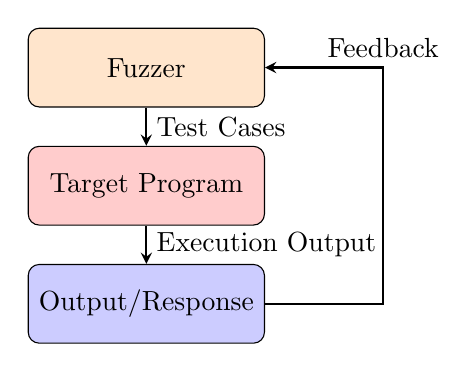
\begin{tikzpicture}[node distance=1.5cm]
                % Define styles for nodes and arrows
        \tikzstyle{box} = [rectangle, rounded corners, minimum width=3cm, minimum height=1cm, text centered, draw=black, fill=blue!20]
        \tikzstyle{fuzzer} = [rectangle, rounded corners, minimum width=3cm, minimum height=1cm, text centered, draw=black, fill=orange!20]
        \tikzstyle{target} = [rectangle, rounded corners, minimum width=3cm, minimum height=1cm, text centered, draw=black, fill=red!20]
        \tikzstyle{arrow} = [thick,->, >=stealth]
        \tikzstyle{title} = [rectangle, rounded corners, minimum width=5cm, text centered, draw=none, fill=none, font=\large\bfseries] 
    
        \node (fuzzer) [fuzzer] {Fuzzer};
        \node (target) [target, below of = fuzzer] {Target Program};
        \node (output) [box, below of = target] {Output/Response};

        % Arrows
        \draw  [arrow](fuzzer) -- (target) node[midway, right] {Test Cases};
        \draw [arrow] (target) -- (output) node[midway,right] {Execution Output};
        \draw [arrow] (output.east) --+(1.5,0) |- (fuzzer.east) node[midway, above] {Feedback};
    \end{tikzpicture}

\end{minipage}
&
\begin{minipage}{\dimexpr0.5\textwidth-2\tabcolsep}
\centering

    % Left Diagram - White Box Fuzzing
    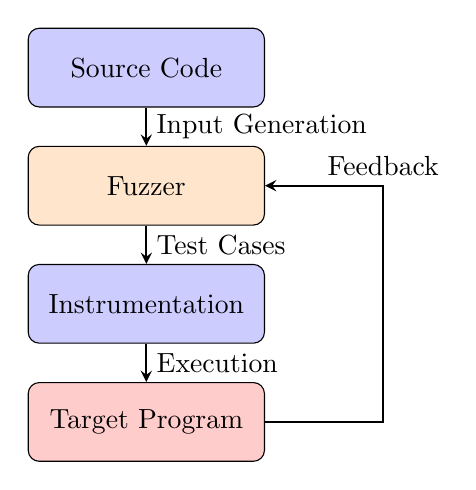
\begin{tikzpicture}[node distance=1.5cm]

        \tikzstyle{box} = [rectangle, rounded corners, minimum width=3cm, minimum height=1cm, text centered, draw=black, fill=blue!20]
        \tikzstyle{fuzzer} = [rectangle, rounded corners, minimum width=3cm, minimum height=1cm, text centered, draw=black, fill=orange!20]
        \tikzstyle{target} = [rectangle, rounded corners, minimum width=3cm, minimum height=1cm, text centered, draw=black, fill=red!20]
        \tikzstyle{arrow} = [thick,->, >=stealth]
        \tikzstyle{title} = [rectangle, rounded corners, minimum width=5cm, text centered, draw=none, fill=none, font=\large\bfseries]
        \node (source) [box] {Source Code};
        \node (fuzzer) [fuzzer, below of = source] {Fuzzer};
        \node (instr) [box, below of = fuzzer] {Instrumentation};
        \node (target) [target, below of = instr] {Target Program};

        % Arrows
        \draw  [arrow](source) -- (fuzzer) node[midway, right] {Input Generation};
        \draw  [arrow](fuzzer) -- (instr) node[midway, right] {Test Cases};
        \draw  [arrow](instr) -- (target) node[midway, right] {Execution};
        \draw  [arrow](target.east) -- +(1.5,0) |- (fuzzer.east) node[midway, above] {Feedback};

    \end{tikzpicture}
    
\end{minipage}

\\

\begin{minipage}[t]{\dimexpr0.5\textwidth-1\tabcolsep}
\captionof{figure}{Simplified black-box fuzzing process}
    \label{fig:black-box-testing}

\end{minipage}
&
\begin{minipage}[t]{\dimexpr0.5\textwidth-1 \tabcolsep}
\captionof{figure}{Simplified white-box fuzzing process}
\label{fig:white-box-testing}

\end{minipage}

\end{tabular*}

\subsubsection{Black Box Fuzzing}
\label{sec:black-box}
\textit{Black box fuzzing} (ref. \autoref{fig:black-box-testing}) is a software testing method that evaluates an application’s security and robustness by feeding it random or semi-random inputs without any knowledge of its internal workings—such as source code, data structures, or algorithms. This approach simulates an external attacker's perspective, enabling testers to discover vulnerabilities that might be exploited by malicious users in a real-world scenario.

The key characteristic of black-box fuzzing is its lack of insight into the internal design and logic of the software being tested. Instead, the focus is on the inputs and outputs of the application. Testers generate a wide variety of input data, often using automated tools or scripts, to gauge how the application responds. This can include testing edge cases, invalid inputs, or unexpected data formats to determine how robust the application is against improper use.

One of the main advantages of black-box fuzzing is its simplicity and ease of use. Since testers do not need to understand the details of the application’s code, they can quickly implement fuzzing without extensive knowledge of the underlying logic. This makes black-box fuzzing an attractive option for assessing third-party software or legacy applications where source code is not available.

Black-box fuzzing can be effective in identifying common security vulnerabilities, such as buffer overflows, input validation errors, and unexpected crashes. By observing how the application behaves with various inputs, testers can pinpoint areas of insecurity, allowing developers to focus their remedial efforts on the most critical issues.

Though black-box fuzzing offers valuable insights into application security, it does have some limitations. Specifically, the randomness of the generated inputs might not exercise all potential execution paths, leaving some vulnerabilities undiscovered. Moreover, in the absence of an understanding of the internal code structure, it may prove challenging to determine which vulnerabilities are of greater significance based on their potential impact.
 \cite{godefroid_random_2007}

\subsubsection{White Box Fuzzing}
\label{sec:white-box}
\textit{White box fuzzing} (ref. \autoref{fig:white-box-testing}) is a software testing technique that seeks to identify vulnerabilities and bugs within applications by utilizing an in-depth understanding of their internal structures and logic. Unlike traditional black-box testing methods, where testers approach the software without any knowledge of its internal workings, white-box fuzzing leverages access to the source code, algorithms, and data flows, allowing for a more targeted and effective analysis.

One of the primary benefits of white-box fuzzing is its ability to generate test inputs based on the actual paths and branches present in the code. By analysing the control flow and data structures inherent to the application, a white-box fuzzer can create specific input cases that exercise various execution paths. This targeted approach increases the likelihood of uncovering potential weaknesses, particularly in areas of the code that may be prone to errors or security vulnerabilities.

Additionally, white-box fuzzing often incorporates dynamic analysis. More on that in ~\autoref{sec:dse}. During the fuzzing process, the application is executed in a controlled environment, and its behaviour monitored in real-time. This provides valuable feedback on how the program reacts to the generated inputs, enabling the identification of unhandled cases that may lead to crashes, incorrect outputs, or security flaws.

Another critical feature of white-box fuzzing is coverage measurement. By measuring code coverage, testers can ensure that their input generation strategies are effective in exercising different paths within the software. This helps identify areas of the code that have not been adequately tested, enabling a more comprehensive examination of the program's reliability and security.

The primary objective of white-box fuzzing is to detect issues such as buffer overflows, null pointer dereferences, and other runtime errors that could compromise an application’s stability or allow for security breaches. By identifying these vulnerabilities early in the development process, organizations can address them proactively, ultimately enhancing the overall quality and security of their software.\cite{godefroid_random_2007}




\subsection{Dynamic Symbolic Execution}
\label{sec:dse}
\textit{Dynamic symbolic execution} (DSE), first presented in the seventies, is a form of white-box fuzzing, as it requires access to the source code. However, instead of requiring an actual input, it assumes that the variables are “symbolic”, meaning that they do not possess a tangible value during execution of the program. Instead, it tracks the conditions encountered during runtime, generating constraints based on the symbolic variables. 
This facilitates a comprehensive examination of multiple program pathways, thereby aiding in the identification of anomalies that may result in unforeseen behaviour or security vulnerabilities.
\cite{boyer_selectformal_1975}\cite{king_new_1975}\cite{king_symbolic_1976}\\
After exploring a particular execution path, DSE employs constraint solvers to analyse the constraints collected during execution. These solvers determine concrete inputs that can satisfy the path constraints, allowing the generation of specific test cases to trigger particular code paths during subsequent executions.

By using DSE, testers can automatically generate test cases that reliably expose bugs or vulnerabilities, such as buffer overflows or access violations. This allows for a more exhaustive testing process that can reveal flaws that traditional fuzzing techniques might overlook.

The synergy between DSE and white-box fuzzing promotes automated test generation and increases the coverage of tested paths, ultimately improving the software's reliability and security. It provides developers with concrete inputs that reproduce identified vulnerabilities, facilitating debugging and remediation.



\subsubsection{Example Dynamic Symbolic Execution}
In this subsection, we will demonstrate the concept of DSE by employing the following code snippet (\autoref{fig:example-program}). 


\vspace{0.5cm}

\begin{tabular*}{\textwidth}{@{}c|c@{}}
    
\begin{minipage}{\dimexpr0.5\textwidth-2\tabcolsep}
\centering
    % Left Diagram - White Box Fuzzing

\begin{lstlisting}[language=JavaScript, gobble=4, escapechar=@]
    function g(x, y) {
        if (x !== y){
            x += y
        }
        else {
            if (y > 8){
                y+=1
            }
        }
        x += 1
        if (x != 0 )
        { 
          if ( y != 0){
            x = y
          }
        }
    }
\end{lstlisting}
   
\end{minipage}
&
\begin{minipage}{\dimexpr0.5\textwidth-2\tabcolsep}
\centering
     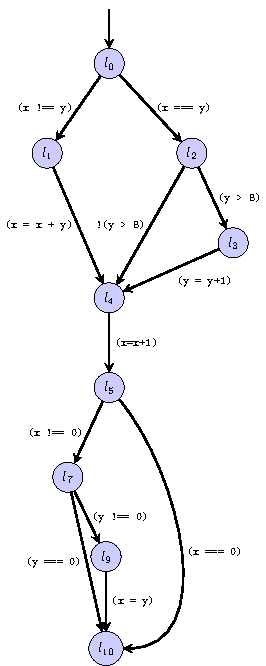
\includegraphics{../luatex/cfg/out/cfg.pdf}
\end{minipage}

\\

\begin{minipage}[t]{\dimexpr0.5\textwidth-1\tabcolsep}
 \captionof{figure}{A simple program}
\label{fig:example-program}

\end{minipage}
&
\begin{minipage}[t]{\dimexpr0.5\textwidth-1 \tabcolsep}
\captionof{figure}{CFG of \autoref{fig:example-program}}
\label{fig:example-program-graph}

\end{minipage}

\end{tabular*}
To facilitate the process, we can first depict the program as a Control Flow Graph (CFG) \autoref{fig:example-program-graph}. 
The CFG displays the conditions and transformations along its edges, with the vertices signifying the state of the program.
On entering  the program, we assume that the initial value of x=1 and y=0, just to tell the DSE Engine the types of the variables, and to give a starting point. 

\begin{center}
    We can denote this as a tuple of (pc, S(x), C(x)) 
    \begin{table}[h]
        \begin{tabular}{lll}
            where & pc & the path condition \\
             & $S(x) \rightarrow X$& the symbolic value of x, i.e. the applied transformations on the initial value\\
             & $C(x) \rightarrow 0$& the concrete value of x\\
        \end{tabular}
    \end{table}
\end{center} 
In similar fashion, we can now walk through the execution, and create a branch whenever we encounter diverging paths.
For example, right at the start, we have two possible routes the execution can take: $x == y$ and $\neg(x == y)$.
We can now construct the symbolic execution tree displayed in \autoref{fig:symbolic-execution-tree} by tracking the path conditions and transformations of the variables.

\begin{sidewaysfigure}
  \centering
  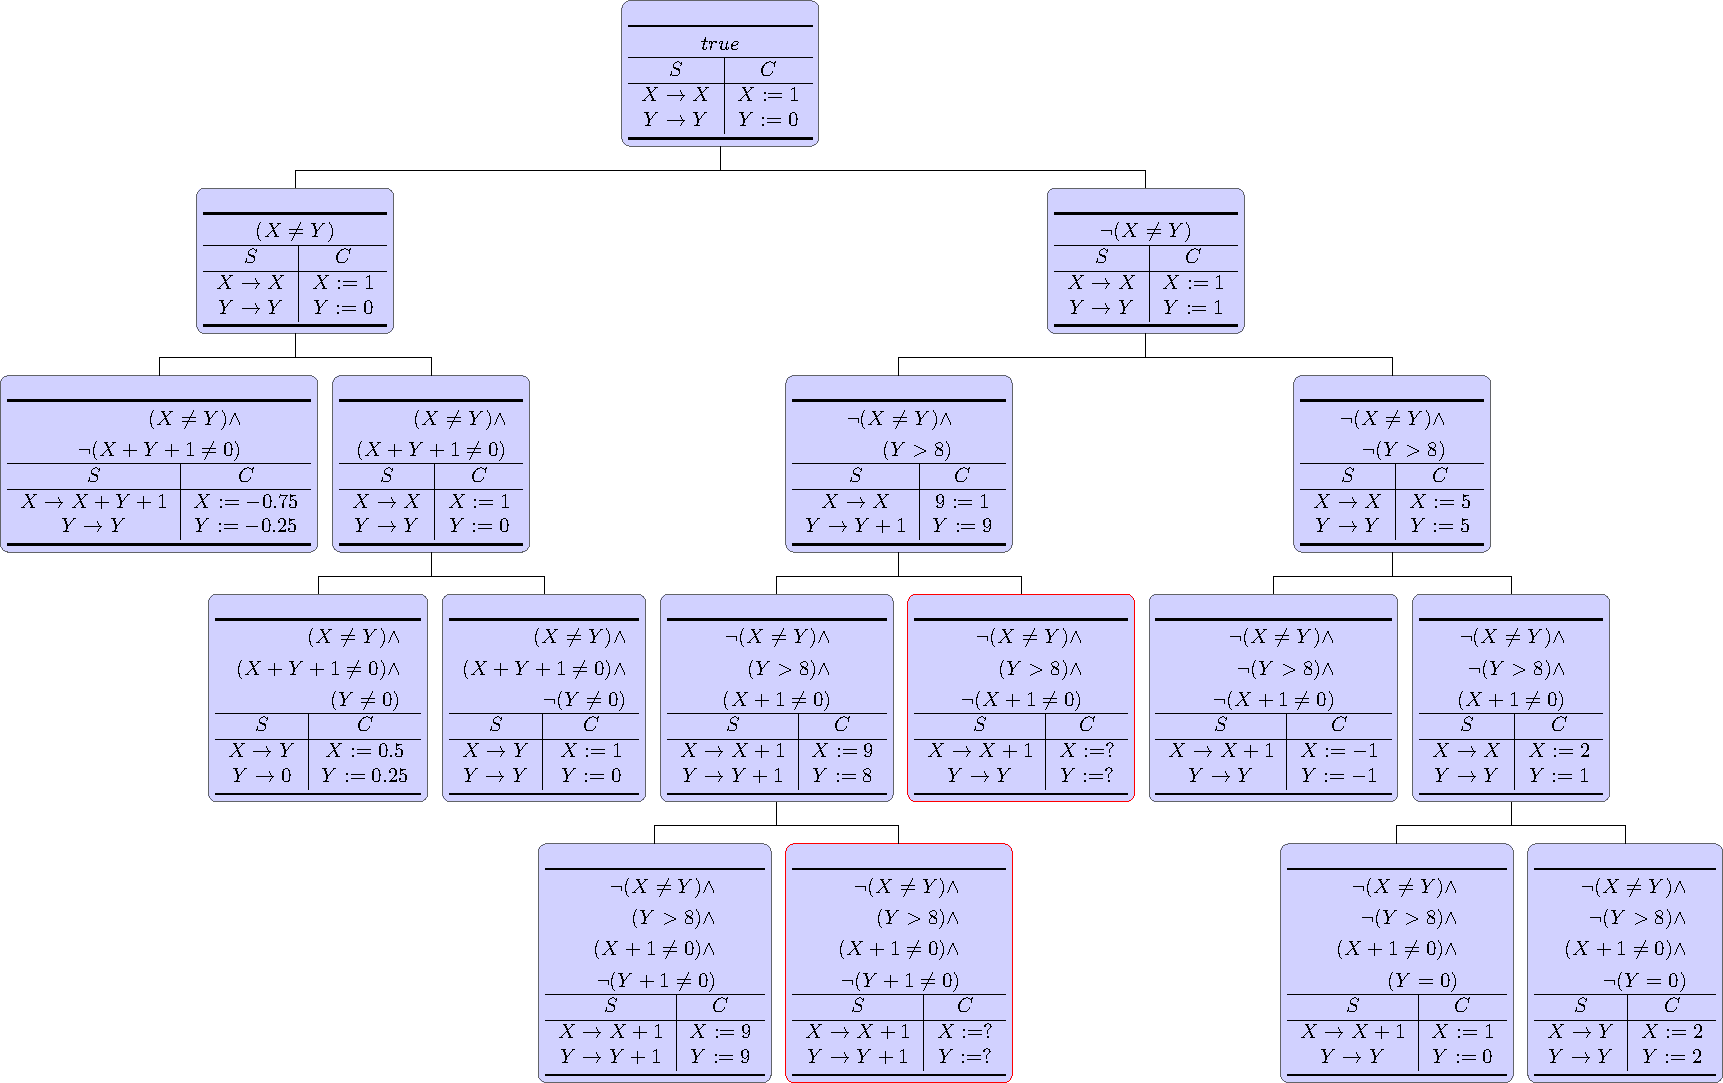
\includegraphics[width=\textwidth]{../luatex/symexe/out/symexe.pdf}    
  \caption{Symbolic execution tree of \autoref{fig:example-program} , displaying the path condition and the concolic state. Unreachable paths are highlighted in red.}
  \label{fig:symbolic-execution-tree}
\end{sidewaysfigure}




After constructing the execution tree, we can generate distinct inputs for each of the leaf nodes, checking for satisfiability.
For instance, if we want to determine which input would cover the branch in the middle of the tree, we can do so by solving the constraints  $(\neg(X \neq Y) \land (Y > 8) \land \neg( X+1==0 ) \land \neg(Y+1 \neq 0 ))$. 
Solving these constraints yields the answer of (x = 9, y = 9), which indicates that this input will satisfy the specified conditions for that branch. 
Any condition that cannot be satisfied means that the leaf node cannot be reached no matter the input. The two leafs highlighted in red in  \autoref{fig:symbolic-execution-tree} showcase this.
These constraints are usually solved by an SMT Solver, which we will briefly explain in \autoref{sec:smtsolver}.


JavaScript has a few peculiarities, as it is dynamically typed and therefore only resolved at runtime. 

\subsubsection{Limitations DSE}

As with any explorative system, DSE has limitations regarding its capabilities. 
The most significant limitation is computable paths, which have the potential to explode if the analysed program is not designed with DSE in mind, for instance, if it heavily relies on recursive calls. 
But even with DSE in mind, the paths grow exponentially with the number of conditionals in a program.  \cite{cadar_symbolic_2013}
This also occurs with symbolic addresses, as it has to account for any possible memory address a variable can occupy \cite{elkarablieh_precise_2009}.  

To address this, most DSE frameworks employ various kinds of techniques for reducing the number of paths. 
One such technique is path merging based on heuristics, where a reoccurring conditional, can be merged into one (for example in a loop)   cite statemerging kinder%TODO
\citet{cha_unleashing_2012} propose a solution for reducing the possible paths for symbolic addresses by concretizing writes and only allowing sybolic.    

It also is not suitable for boundary testing, as DSE checks for reachability, and once a path is covered, it will not move back and check for edge case in this path, possibly missing unexpected behaviour. \cite{berthier_efficient_2023}


\FloatBarrier
\subsection{SMT Solver}
\label{sec:smtsolver}

A \textit{satisfiability modulo theories }(SMT) Solver is a tool used in formal verification, automated reasoning, and various applications within computer science and engineering. The need for SMT solvers arises from the complexity of verifying whether certain logical formulas, particularly those involving rich theories such as integers, real numbers, arrays, and others, are satisfiable. Traditional propositional satisfiability (SAT) solvers face challenges with these complex theories, which is why the development of SMT solvers has become essential for enhancing automated reasoning capabilities.

SMT solvers extend the capabilities of SAT solvers by incorporating various decision procedures tailored for different theories. The process begins with the translation of a given problem into a logical formula that can be expressed in a first-order language. Initially, the SMT problem is transformed into a conjunction of logical formulas, some of which may involve theoretical constructs. Each theory, such as those pertaining to integers, arrays, or bit-vectors, possesses its own decision procedure. SMT solvers combine these procedures to handle the entire formula, typically through a technique known as "dPLL(T)," where T represents the specific theory being addressed.


When an SMT solver processes a logical formula, it checks for potential conflicts—instances in which segments of the formula cannot be simultaneously satisfied. If a conflict is detected, the solver uses conflict analysis to learn from this situation and backtrack efficiently to explore other possibilities. Throughout this process, the solver iteratively refines its search, evaluating potential assignments to variables while ensuring consistent adherence to the theoretical constraints at hand. This harmonious integration of modular theory solvers with SAT-like search techniques allows SMT solvers to effectively determine the satisfiability of complex logical formulas.\cite{barrett_satisfiability_2009}



Notable SMT solvers, such as Z3 and CVC5, have significantly impacted the field. The Z3 SMT solver, which is utilized as an SMT Solver for expoSE and was developed by Microsoft Research, has gained widespread acceptance and provides robust support for numerous theories. CVC5, developed at Stanford University, emphasizes efficiency in its decision procedures. Advances in automated reasoning have helped to establish SMT solvers as essential components in many formal verification tools, program analysis frameworks, and synthesis technologies.\cite{barrett_satisfiability_2009}


\section{Tech Stack}
\label{sec:tech}
In this section, we will delve into the inner workings of the expoSE framework, what tools it uses and their function within. 
For the following sections, we will use the following small code snippet to explain how the system works. 


\begin{figure}[h]
    \begin{lstlisting}[language=JavaScript, gobble=4]
    const S$ = require("S$");
    

    let x = S$.symbol("value"); 
    let y = S$.symbol("multiplier", 2);
    
    if (x > 0) {
        S$.assert(x*y > x, "assertion violation"); 
    }
    
   
    \end{lstlisting}
    \caption{A simple program for ExpoSE}
    \label{fig:expose-sample-program}
\end{figure}



\subsection{Jalangi}
\label{sec:jalangi}
"Jalangi2 is a framework for writing dynamic analyses for JavaScript." \cite{noauthor_samsungjalangi2_nodate}\\
Jalangi2, first presented in \citet{sen_jalangi_2013}, is used to instrument the JavaScript code that is to be analysed and provides callbacks for a program to spy onto the execution.
It enables this, by attempting to simplify every execution statement by breaking them down into atoms, which are made up of the functions listed \autoref{tab:jal-fun}, which in turn provide callbacks to hook further into the execution.
The analysing tool can implement these callbacks in order to gain insight and/or modify the return value.


To instrument the code snippet in \autoref{fig:expose-sample-program}, Jalangi2 first transforms the passed code to es6 using Babble, to ensure a consistent syntax. 
Afterward, Jalangi2 instruments the code using the JavaScript parser "acorn"\footnote{https://github.com/acornjs/acorn} to generate the AST (Abstract Syntax Tree) and then rewrites the code using Jalangi's own operatrions. This creates two files per input: 
A \{filename\}\_jalangi.js and a \{filename\}\_jalangi.json. The .js file, contains the instrumented code, similar to \autoref{fig:code-snippet}, along with the static unique instruction identifiers (iids) of each callback as a JSON object, while the .json file only contains the iids.

Although the functions exhibit variation in their parameters, they always include the iid (instruction identifier) as their primary parameter. This identifier serves as a unique reference within a JSON object, which stores an array for each statement. Each array contains critical metadata consisting of the starting line number, the column of the expression on that line, the line number where the expression concludes, and the respective column number associated with the termination of the expression.



\begin{figure}[ht]

 \lstset{basicstyle=\footnotesize}
    \begin{lstlisting}[language=JavaScript, gobble=4]
    J$.N(225, 'S$', S$, 0);             // Init S$
    J$.N(233, 'x', x, 0);               // Init x
    J$.N(241, 'y', y, 0);               // Init y
    var S$ = J$.X1(41,                  // Top level declaration
        J$.W(33, 'S$',                  // Write the result of the following:
            J$.F(25,                 // Call the function with the follwing parameter:
                J$.R(9, 'require', require, 2),// Read the value of "require"
                0)  (
                    J$.T(17, "S$", 21, false)    // Retrieve the value of the S$ object
                    ), S$, 3));
    var x = J$.X1(89,                            // Top level declaration
        J$.W(81, 'x',                            // Write the result of the following:
            J$.M(73,                                   // Call the function of:
                J$.R(49, 'S$', S$, 1),           // Read the value of the expression S$
                'symbol', 0)                     // Name of the called function
                    (J$.T(57,"value", 21, false),// Defines the value of the 
                                                 // variable as literal
            J$.T(65, 0, 22, false)),x, 3));      // Retrieve the value "0"


    \end{lstlisting}
    \caption{A shortened program snippet from \autoref{fig:expose-sample-program}, instrumented by JALANGI2, with explanation}
    \label{fig:code-snippet}
\end{figure}

As it is apparent in \autoref{fig:code-snippet}, every assignment can be traced on a granular level, enabling the analyser to know the exact state of a program, at any stage of the execution. 
If, for example, we wanted to modify, or simply log the value of the multiplier in line 24, we could do so by hooking (accessing the execution process) into the callback function provided for the function T.
This example, of course, is almost as simple as it can get. This is because JavaScript is known for having expressions that contain multiple callbacks, which in turn may or may not have callbacks themselves, colloquially called “Callback Hell” \cite{max_ogden_callback_2019}. And while an example with a callback would be a better representation of a real program, it would also mean that the instrumented code example be by a magnitude longer, rendering the example incomprehensible (not to mention, \textit{rendering} it on PDF and having it readable impossible). \\


\begin{table}[h]
\resizebox{\linewidth}{!}{%
	\begin{tabular}{l|l|l}
    {\lstinline|J$.U           |} & Unary operation                                       & {\lstinline|unaryPre|} and {\lstinline|unary|}                      \\
		{\lstinline|J\$.B           |} & Binary operation                                      & \lstinline|binaryPre| and \lstinline|binary|                    \\
		{\lstinline|J\$.C           |} & Condition                                             & \lstinline|conditional|                             \\
		{\lstinline|J\$.C1          |} & Switch key \lstinline|x in switch(x) { ... }|                    & no callback                             \\
    {\lstinline|J\$.C2          |} & case label \lstinline|C1 === C2|                                  & no own callback, uses callback of {\lstinline|J\$.C|} \\
		{\lstinline|J\$.\_          |} & Last value passed to C                                & no own callback                         \\
    {\lstinline|J\$.H           |} & hash in for-in. Wrap object \lstinline|o in for (x in o) { ... }| & {\lstinline|forinObject|}                             \\
  {\lstinline|J\$.I           |} & Ignore argument (Identity)                             & no callback                             \\
		{\lstinline|J\$.G           |} & Get a field                                              & \lstinline|getFieldPre| and \lstinline|getField|                \\
		{\lstinline|J\$.P           |} & Put a Field                                             & \lstinline|putFieldPre| and \lstinline|putField|                \\
		{\lstinline|J\$.R           |} & Read variable                                         & \lstinline|read|                                    \\
		{\lstinline|J\$.W           |} & Write variable                                        &\lstinline|write |                                  \\
		{\lstinline|J\$.N           |} & Init                                                  &\lstinline|declare|                                 \\
		{\lstinline|J\$.T           |} & object/function/regexp/array Literal                  &\lstinline|literal |                                \\
		{\lstinline|J\$.F           |} & Function call                                         &\lstinline|invokeFun|                               \\
    {\lstinline|J\$.M           |} & Method call                                           &\lstinline|invokeFun| and uses callbacks of {\lstinline|J\$.P|}   \\
		{\lstinline|J\$.A           |} & Modify and assign \lstinline|+=, -= ...|                          & uses callbacks of \lstinline|J\$.P| and \lstinline|J\$.B|       \\
		{\lstinline|J\$.Fe          |} & Function enter                                        &\lstinline| functionEnter |                          \\
		{\lstinline|J\$.Fr          |} & Function return                                       &\lstinline| functionExit  |                          \\
		{\lstinline|J\$.Se          |} & Script enter                                          &\lstinline| scriptEnter   |                          \\
		{\lstinline|J\$.Sr          |} & Script return                                         &\lstinline| scriptExit    |                          \\
		{\lstinline|J\$.Rt          |} & returned value                                        &\lstinline| \_return      |                          \\
		{\lstinline|J\$.Th          |} & thrown value                                          &\lstinline| \_throw       |                          \\
		{\lstinline|J\$.Ra          |} & Reads the return value stored by call to \lstinline|Rt()|         & no callback                             \\
		{\lstinline|J\$.Ex          |} & Uncaught exceptions                                   & no callback                             \\
		{\lstinline|J\$.L           |} & Returns the last computed value                       & no callback                             \\
		{\lstinline|J\$.X1          |} & top level expression                                  &\lstinline| endExpression               |            \\
		{\lstinline|J\$.Wi          |} & with statement                                        &\lstinline| \_with                      |            \\
		{\lstinline|J\$.endExecution|} & terminating execution                                 &\lstinline| endExecution                |            \\
		{\lstinline|J\$.S           |} & with statement                                        &\lstinline| runInstrumentedFunctionBody |            \\
	\end{tabular}}
	\caption{Jalangi2  functions, their descriptions, and their callbacks as stated in the JavaScript Documentation of the analyser}
	\label{tab:jal-fun}
\end{table}

\FloatBarrier
\subsection{Z3 SMT Solver and Z3JavaScript}
\label{sec:z3}


ExpoSE uses the Z3 SMT Solver \cite{de_moura_z3_2008} for solving the found path conditions of the analysed program. Developed by Microsoft, it has constant progress and improvements to its capabilities.

To use the SMT Solver, it offers an interface that connects a program in a higher-level language, like Python, Java, C++, or JavaScript, for which z3 offers a NPM (Node Package Manager) package since 2022. In expoSE, however, it is used in combination with the project Z3JavaScript, as, when expoSE got developed, there were no native JavaScript bindings available for Z3. 

These bindings are required to connect these higher-level languages to the core system of z3, which is implemented in C.

ExpoSE uses it to solve the path conditions generated by the first run of the symbolic execution, to yield new inputs, which in turn add new path conditions to be solved by Z3. 


Z3Javascript is a wrapper for the API of Z3, which generates the JavaScript bindings to be used in ExpoSE using ffi-napi, and builds the Z3 binary.

It then exposes functions that are used to interact with Z3, converting JavaScript types into C-types. 
Additionally, it transforms JavaScript regular expressions in order for the Z3 parser to understand them.






\newpage
\subsection{expoSE}
\label{sec:expose}
So, what exactly is ExpoSE? \\
In short, it is a DSE Framework for JavaScript, which allows almost any JavaScript code to be tested for bugs, generate tests that cover the code base to a high degree and checks for reachability of statements, by employing the aforementioned tools. \cite{loring_expose_2017}

In the following, we will demonstrate how exactly the framework operates. \\
Assume we have a small function:\\
Now, while short, there already is a lot to unpack here. Let's go over it line by line. 
\begin{itemize}
    \item Line 1: \lstinline{const S$ = require("S$")}: S\$ loads the interface library, that allows the user to interact with expoSE, declare a variable as symbolic and create assertions of conditions. More on that in the next lines.
    \item Line 3: \lstinline{let x = S$.symbol("value")}: We create a symbolic variable "x" by using the S\$ function "symbol", which allows us to define a name to track the variable with. We pass the systenm internal variable name "value" as parameter.  
    \item Line 4: \lstinline{let y = S$.symbol("multiplier", 2)}: We then create a symbolic variable “y”, internally called “multiplier”, this time, we also assign a starting seed (2), which at the same time defines the type of the variable.
    \item Line 5 to 7: then apply these variables and try to do something with them. Here, we have a simple condition ($x > 0$), which, when fulfilled, triggers the assertion \lstinline{S$.assert(x*y > x)}, which throws the exception “assertion violation”, if  the assertion is violated.
\end{itemize}
Afterwards, expoSE uses the functions exposed by the Jalangi2 backend  to access the instrumented code. For this, expoSE had to implement the callbacks of the provided backend functions. A template for these can be found in the Jalangi2 source code, with explanations for each of the functions, as part of an example analysis program\footnote{https://github.com/Samsung/jalangi2/blob/master/src/js/runtime/analysisCallbackTemplate.js}. 
It starts by registering all local variables, functions and formal parameters, in our example case the variables and constants S\$, x and y. Subsequently, it resolves the statements, loads the S\$ library and creates a concolic variable: if a concrete value is present, it uses this as starting seed. Otherwise, it will try all primitive types as the first input generation (i.e. string, array, number, object etc). The symbolic part of the concolic wrapper saves all encountered path conditions, which will be used to generate a new input which satisfies another path condition, thereby diverging from the original path, and maybe finding alternative paths.
By having the assertion \lstinline{x*y > x} we force ExpoSE to create two more paths than it normally would. Without the assertion, there are the two paths \lstinline{x>0} and \lstinline{!x>0}. But with the assertion, we added the path condition \lstinline{(x*y) > x} and its negation. This can be used to test for a certain behaviour, but requires manual modification of the program. Similar to normal conditionals, it also leads to the amount of explorable paths to explode.
